\chapter{General Characteristics of the New Zealand Flora}

The current estimate for the number of vascular plant species native to New Zealand is about 2200.\footnote{\cite{druce1984indigenous}}
This is a modest total by comparison with tropical floras, but it is of moderate size for a temperate country.
About 82 per cent of the species are endemic; a high proportion reflecting New Zealand's isolation.

New Zealand is a generally moist country with mild temperatures in the lowlands.
It is believed that before human habitation much of the landscape was covered by dense forests --- conifer broadleaf\footnote{Broadleaf is a term applied to flowering plants (angiosperms), whose leaves are usually much wider than those of conifers.} forest predominating in the warmer North Island and parts of the South Island and beech (\BotanicRef{Nothofagus}) forest predominating in the South Island and, mostly at higher altitudes, in the North Island.
Human activities have greatly reduced this forest cover.
Above treeline, ranging north to south from about \SIrange{1500}{1000}{\metre} in altitude, there are various types of short alpine vegetation, which sometimes include a belt of shrubs as a transition from the forest\figureref{\fullref{fig:1vegetationpatterns}}.

\afterpage{%
	\begin{figure}[!t]
		\centering
		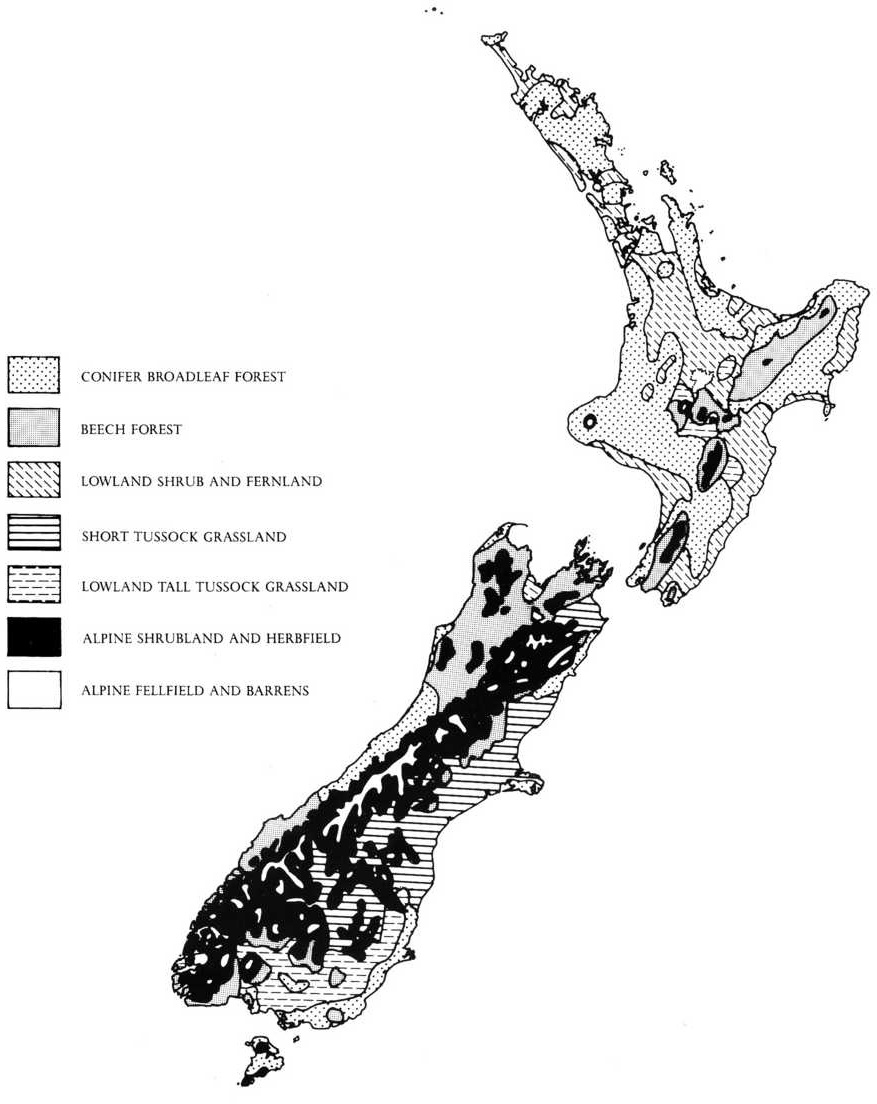
\includegraphics[width=0.8\textwidth]{graphics/figure1vegetation-patterns.jpg}
		\caption[Broad patterns of vegetation]{The broad patterns of vegetation at the time of European settlement in New Zealand in the 19th Century. 
		It is believed that the areas of fern and shrubland, short tussock grassland and lowland tall tussock grassland were largely forested before the Maori settled in New Zealand 1000 years earlier. 
		This is discussed in Chapter~\ref{ch:openhabitats} \nameref{ch:openhabitats}.}%
		\label{fig:1vegetationpatterns}
	\end{figure}
}

Of the world's larger islands, New Zealand's narrowly separated pair are the most remote from any continent.
The British Isles and Japan are as close to their adjacent continents, at their nearest points, as the North and South Islands are to each other; the larger islands of Indonesia and the Caribbean form close set series between continents and even Madagascar is, at 400 kilometres from Africa, only one quarter the distance from that continent that New Zealand is from Australia, its nearest continental neighbour.

Most of New Zealand's rocks are sedimentary, laid down originally beneath the sea, and as a basis for our understanding of the history and characteristics of the flora we need to know whether New Zealand emerged in its present isolation or whether it was first connected with a larger landmass.

Before considering what geologists have to say on this point we will see whether the plants themselves can tell us anything.
Do floras which have evolved on isolated islands which have never been connected to a continent have any characteristics to distinguish them from continental floras? Studies of both the flora and fauna of Hawai{\okina}i,\footnote{\cite{carlquist1970hawaii}} as well as of other isolated islands,\footnote{\cite{carlquist1965island}} suggest that the answer to this question is `yes'

\section[The Isolated Island Syndrome]{The Isolated Island Syndrome\thinspace\footnote{\cite{ehrendorfer1979reproductive}}\footnote{\cite{lloyd1985progress}}}

The area of the Hawaiian islands is much less than that of New Zealand but their isolation is much greater, since the nearest continent, North America, is \SI{4000}{\kilo\metre} distant and both Australasia and Asia are about \SI{7000}{\kilo\metre} distant.
The Hawaiian islands are entirely volcanic and have arisen sequentially on a north-west to south-east line over the last 4 to 5 million years.
Hawai{\okina}i, the southernmost island, is thus the youngest and is also the largest and highest (\SI{4000}{\metre}).
There seems little possibility, geologically, that these islands have ever been connected to a continent, so botanists and zoologists alike envisage their being stocked by chance immigrants with subsequent evolution of new species.
Thus it has been estimated that 272 immigrant species could have evolved into the present approximately 1200 native higher plant species of Hawai{\okina}i.
The distinguishing characteristics of floras that have been derived in this way can be outlined as follows:

\subsection{Getting There}

Not unexpectedly, plant and animal groups with good dispersal ability are strongly represented, while those with poor dispersal ability are absent.
Among plants, those with seeds that have special modifications for dispersal (for example: flotation devices for sea transport; plumes of hairs for wind dispersal; hooks for attachment to birds' feathers; or hard seeds in berry fruits eaten by birds and eventually excreted intact), have a good chance of eventually reaching an isolated island.
Plant groups which are notable for not reaching such islands, because their seeds are large and/or unspecialised, include conifers; the wind pollinated trees (including oaks and beeches, so important in some temperate forests of the northern hemisphere); and most of the primitive woody flowering plant families in the order Ranales, of which \BotanicRef{Magnolia} is the best known example.
Prominent among animals on isolated islands are those with wings --- birds and insects --- while mammals, amphibians and land reptiles are absent.

Strangely, many species of small, isolated islands have lost or have only vestiges of the dispersal mechanisms possessed by their continental relatives.
Thus there are many flightless island birds and insects.
Among plants, species belonging to groups that are normally wind dispersed may have seeds with quite inadequate vestigial wings or plumes of hairs.
In explanation of this it has been suggested that, although a good dispersal mechanism is necessary for a plant species to reach an isolated island, once the plant is established, good dispersability would become a disadvantage for most of the seeds would end up uselessly in the sea!

\subsection{Adaptive Radiation}

Many genera on isolated islands exhibit a much wider range of growth forms and occupy a much wider range of habitats than the same or related genera on continents.
Thus on mountainous islands like Hawai{\okina}i, some species of a genus may be small and herbaceous and occupy coastal and lowland open habitats, other species may be small trees in wet forests at various altitudes, and yet others shrubs or herbs in alpine vegetation.
Carlquist,\footnote{\cite{carlquist1970hawaii}}\footnote{\cite{carlquist1965island}} who has closely studied island floras and faunas, suggests that the first species of a plant genus to arrive is likely to be a weedy herb, because in general weeds are good dispersers and hardy enough to tolerate the raw open conditions of a new volcanic island.
In such a situation many habitats will remain unoccupied for some time (particularly, Carlquist suggests, those suitable for moist forests), so any variants of the weedy coloniser with habitat requirements different from the parent population would have a very good chance of establishing in an unoccupied niche.
In turn a variant population could give rise to other variants to occupy further niches including, if the island is high enough, those of alpine habitats.
Such a burst of speciation into unoccupied habitats has been termed `adaptive radiation'.
It is not suggested, however, that a species increases its ability to give rise to new varieties and species on migrating from a continent to an isolated island.
On the continent it would also form variants, but these would rarely find unoccupied habitats suited to their needs.

Carlquist's view that weedy herbs are frequently the first colonisers of isolated islands implies a general trend in plant evolution on some islands from herbs to trees.
This is entirely possible, but it would be an unusual direction for evolution to take, if the generally accepted idea that herbs are advanced, relatively recent in origin and derived from woody ancestors, is correct.
In opposition to Carlquist's view some botanists believe that tree species on isolated islands, belonging to genera or even families which are otherwise mostly herbaceous, are primitive ancestral forms that have survived there because of the mild oceanic climates and reduced competition.\footnote{\cite{mabberley1979pachycaul}}
On continents, particularly those of the northern hemisphere, woody species of these groups have generally given way to herbaceous species better suited to the strongly seasonal climates which have developed at higher latitudes on continents in recent geological time.

\subsection{Sexual Patterns}

It would seem obvious that a plant species with self-fertile hermaphrodite flowers would stand a better chance of establishing on an isolated island than an hermaphrodite species which is self-sterile or a species with separate male and female plants, a condition known as dioecism.
In both the latter cases one plant would not be sufficient to form a population; at least two would be required --- one male and one female in the case of a dioecious species --- and they would have to establish at the same place and coincide or overlap in time.
In some cases, however, this might not be unlikely, as in some species seeds tend to be transported in groups.
Berries often contain several small seeds, so a bird might eat a number of berries of a particular species, transport them internally and deposit them in a group on an isolated island.
This could be the case with the dioecious, berry-fruited genus \BotanicRef{Coprosma}, so strongly represented in both the New Zealand and Hawaiian floras.
Sticky or barbed seeds which attach themselves externally to birds or seeds in mud might also be transported in groups, but this would be less likely with seeds conveyed by winds or ocean currents.
Nevertheless, the odds would seem to favour self-fertilising plants as colonisers of isolated islands, and we would expect a lower percentage of say dioecious species on such islands than on a continent.
Paradoxically, the reverse is the case.
In Hawai{\okina}i it is estimated that 27.5 per cent of the species are dioecious,\footnote{\cite{carlquist1970hawaii}} a much higher proportion than for the United Kingdom, for example, where it is estimated only 2 per cent of species are in this category.

How can this be? If dioecious species are less likely to colonise isolated islands and yet are found there in relatively large numbers, there must be some circumstance which especially favours both the survival and diversification of the relatively few dioecious colonisers and the evolution of dioecious from hermaphrodite island species.
This implies that dioecism confers some special advantage in the isolated island situation.
It has been suggested that this advantage results from the obligate outcrossing of dioecious species, which brings about an increase in variability.
Variable species are more likely to be successful on isolated islands as they are in a better position to take advantage of the unoccupied habitats available, and more likely to survive drastic environmental changes such as those resulting from the succession of glacials and interglacials in recent geological time.
On a continent stretching from high to low latitudes, species can survive such fluctuations by migrating with their preferred climates as these climates move towards and away from the equator.
On an isolated island, this option is greatly restricted, so with a drastic environmental change, a greater proportion of relatively invariable inbreeding species will become extinct than of more variable outcrossing species, which are better able to adapt to change.

\subsection{Hybrids}

A similar explanation has been suggested for the high level of natural hybridism on isolated islands.\footnote{\cite{gillett1972role}}\footnote{\cite{rattenbury1962cyclic}} The progeny from such hybrids displays an even greater variability than that resulting from dioecism, and should thus be an even richer source for the populating of unoccupied habitats or new habitats resulting from environmental change.

\subsection{Lack of Brightly Coloured Flowers}

On islands like Hawai{\okina}i an unusually high proportion of the native plants have small, shallow flowers which lack bright colours and are pollinated by wind or unspecialised short tongued insects.
The exceptions are certain bird-pollinated species which have larger red to yellow flowers of tubular form.

The general lack of brightly coloured flowers is attributable to the absence from isolated islands of the more specialised insect pollinators, particularly long tongued bees, which are attracted by bright colours and pleasant perfumes.

\section{The New Zealand Pattern}

Such then is the `isolated island syndrome'.
The question now arises: `does the New Zealand flora also conform to this pattern'? The answer this time is `yes and no'.

The strongest difference from the isolated island pattern lies in the presence in New Zealand, mainly in forests, of plants belonging to groups of poor dispersal ability.

\begin{description}
	\item[{(a)}]Conifers are a prominent feature of the forests with the giant \IDX{kauri} (\BotanicRef{Agathis australis}[Agathis][australis]) in the far north and the more widespread species of the family Podocarpaceae (`Podocarps') including \IDX{rimu} (\BotanicRef{Dacrydium cupressinum}[Dacrydium][cupressinum]), \IDX{kahikatea} (\BotanicRef{Dacrycarpus dacrydioides}[Dacrycarpus][dacrydioides]) and \IDX{totara} (\BotanicRef{Podocarpus totara}[Podocarpus][totara]).
	\item[{(b)}]The largely northern temperate group of wind-pollinated trees is represented in New Zealand by species of southern hemisphere beech (\BotanicRef{Nothofagus}) which form extensive forests at mostly higher altitudes and latitudes.
	\item[{(c)}]The woody families of the order Ranales are represented in New Zealand by several species, including \IDX{horopito} (\BotanicRef{Pseudowintera} species), \IDX{tawa} (\BotanicRef{Beilschmiedia tawa}[Beilschmiedia][tawa]) and \IDX{pukatea} (\BotanicRef{Laurelia novae-zelandiae}[Laurelia][novae-zelandiae]).
\end{description}

The presence of representatives of these and other ancient and mostly southern groups not represented on islands which have always been isolated, indicates that New Zealand has not always been as isolated as it is now and must once have had continental connections.

How, when and where was New Zealand linked to other lands to receive this ancient element? When speculating on this point, proponents of the `land-bridge' theory have made much of the fact that New Zealand is situated on an extensive system of relatively shallow submarine plateaus and ridges --- the Chatham Rise and the Campbell Plateau to the south-east extending to about \ang{55}S and the Lord Howe Rise and Norfolk Ridge to the north-west extending to about \ang{20}S\figureref{\fullref{fig:2crust}}.
Recent evidence suggests that these plateaus and ridges are composed of continental rocks and were once land.
\IDX{New Caledonia}, at the northern end of the Norfolk Ridge, has rocks very similar to those of New Zealand and has an ancient southern element in its flora that is related to but even larger than that of New Zealand.
Thus we have to consider past connections, not just of New Zealand, but of a small and now largely submerged continental landmass of which New Zealand and \IDX{New Caledonia} are the only parts still above sea level.
For convenience of reference this small continent could be termed Tasmantis, a name that has earlier been applied to a hypothetical land in the Tasman Sea region.

\begin{figure}[t]
	% Outer minipage scaled to limit width.
	% Inner minipages scaled so the images have the same height.
	\begin{minipage}[t]{0.9\textwidth}
		\begin{minipage}[t]{(\textwidth-\fgap) * \real{0.62}}
			\centering
			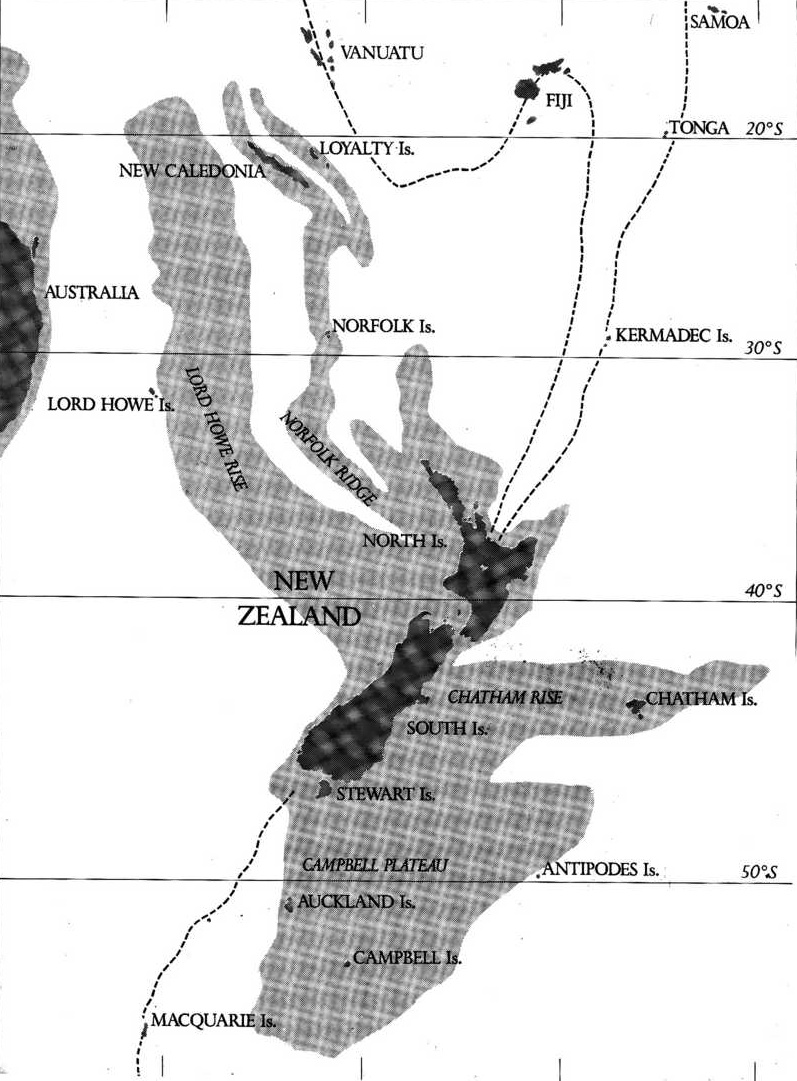
\includegraphics[width=\textwidth]{graphics/figure2crust.jpg}
			\caption[The New Zealand crustal complex]{The New Zealand crustal complex.
			Dark grey: dry land.
			Light grey: submerged continental to subcontinental crust.
			Dashed lines: volcanic ridges.}%
			\label{fig:2crust}
		\end{minipage}\hspace{\fgap}%
		\begin{minipage}[t]{(\textwidth-\fgap) * \real{0.38}}
			\centering
			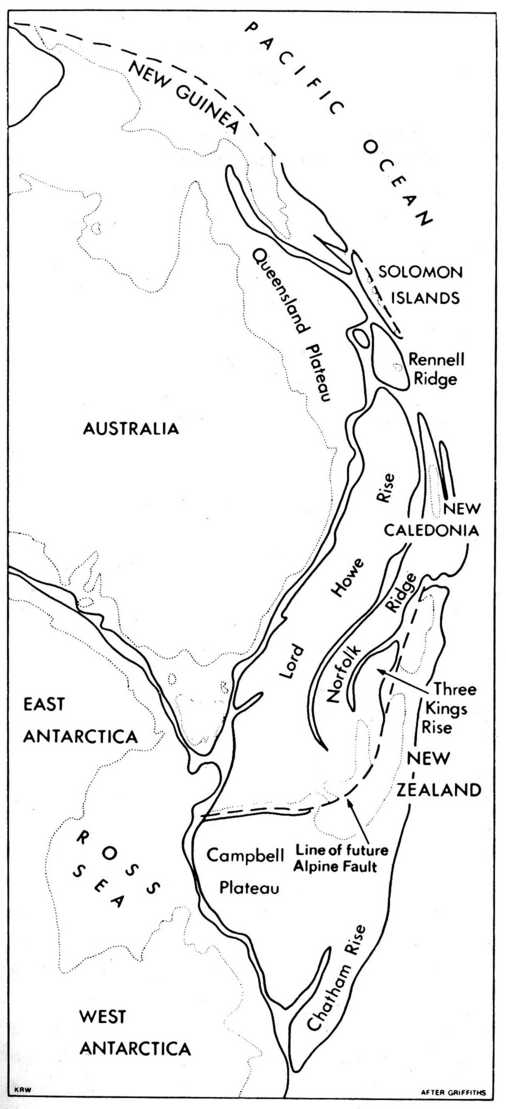
\includegraphics[width=\textwidth]{graphics/figure3gondwana.jpg}
			\caption[Proposed reconstruction of the Australian/Antarctic/Tasmantis portion of Gondwana]{Proposed reconstruction of the Australian/Antarctic/Tasmantis portion of Gondwana during the mid-Cretaceous about 90 million years ago.
			After Tasmantis separated lateral movements along the alpine fault gradually rearranged the crust of present New Zealand.}%
			\label{fig:3gondwana}
		\end{minipage}
	\end{minipage}
\end{figure}

According to the land-bridge theory, then, if Tasmantis were once largely above the sea then dry land may have extended to New Guinea and perhaps even to south-east Asia.
Such a land extension might explain some of our floristic links with the tropics, but not so readily those with the former flora of Antarctica and the present flora of South America, as the \SI{2000}{\kilo\metre} gap between the Campbell Plateau and Antarctica makes it difficult to envisage a former dry land connection between them.

Another theory provides a more likely explanation.
Recent geophysical evidence of sea floor spreading has led to a fairly general acceptance of the old theory of continental drift, with some modification.\footnote{\cite{stevens1980new}}
As far as the southern hemisphere is concerned it is believed that all its land areas, as well as India, were once united in a single large continent known as Gondwana.
India and Africa/South America first separated off and later became separated from each other.
Through its southern extremity South America probably retained tenuous links with the Antarctica /Australia/Tasmantis remnant of Gondwana\figureref{\fullref{fig:3gondwana}}.
It is suggested that Tasmantis separated and moved into isolation about 80 million years ago and that Australia and Antarctica fully separated about 50 million years ago.
If the timing of these separations is correct then the ancient southern floral element could have reached New Zealand and \IDX{New Caledonia} before Tasmantis drifted into isolation.
The presence of this element in the New Zealand flora is the most notable contrast with the floras of isolated islands, but in other respects there are several points of agreement:

\begin{description}
	\item[{(a)}]A number of genera in New Zealand, like many genera of isolated islands, exhibit a wide morphological and ecological range.
	To cite \BotanicRef{Coprosma} again, some species are small trees with large leaves in the lowland forests, others are densely branched small-leaved shrubs mostly of open habitats from the sea coast to above tree-line in the mountains, and a few are mat-forming, near-herbs of the high mountains and montane riverbeds.
	Similar wide ranges are evident in a number of other genera including \BotanicRef{Pittosporum} and \BotanicRef{Myrsine}.
	Even in genera with only a few species in New Zealand there may be an extreme range in growth habit.
	Of our three species of \BotanicRef{Fuchsia} one, \IDX{kotukutuku} (\BotanicRef{Fuchsia excorticata}[Fuchsia][excorticata]) is a small tree, one is a scrambling climber (\BotanicRef{Fuchsia perscandens}[Fuchsia][perscandens]) and the last, \IDX{creeping fuchsia} (\BotanicRef{Fuchsia procumbens}[Fuchsia][procumbens]) is a prostrate, spreading near-herb.
	\begin{SCfigure}[2][!b]
		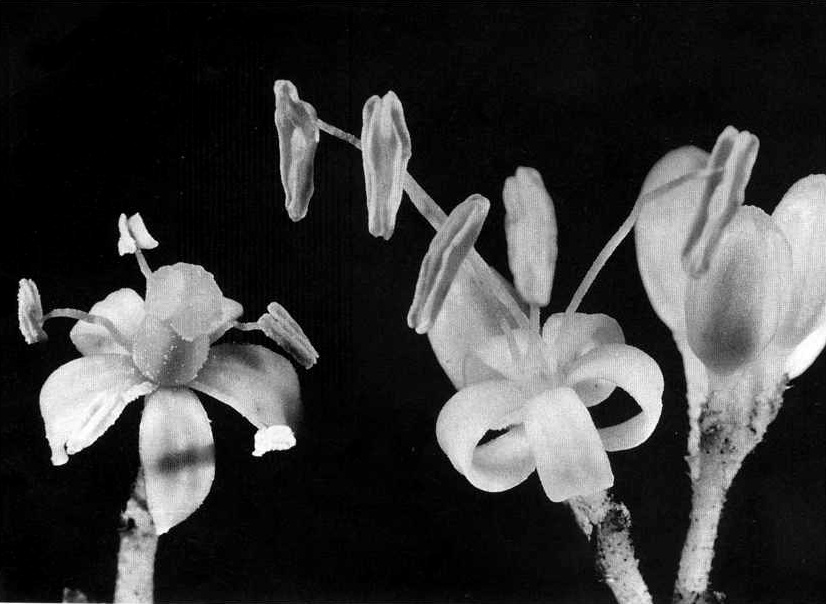
\includegraphics[width=0.66\textwidth]{graphics/figure4kaikomako.jpg}
		\centering
		\caption[Kaikomako: A New Zealand example of dioecism]{\IDX{Kaikomako}[kaikomako] (\BotanicRef{Pennantia corymbosa}[Pennantia][corymbosa]): A New Zealand example of dioecism.
		The female flower on the left has a well developed ovary at the centre, but the small stamens do not produce viable pollen.
		The male flower on the right has only a rudimentary nonfunctional ovary, not discernible in this photo, but has large stamens with long filaments.
		Kaikomako is probably wind-pollinated.
		Photo: B. V. Sneddon.}%
		\label{fig:4kaikomako}
	\end{SCfigure}
	\item[{(b)}]The level of dioecism in the New Zealand flora\figureref{\fullref{fig:4kaikomako}} is, at 12 per cent,\footnote{\cite{godley1979flower}} much lower than that of Hawai{\okina}i, but still much higher than that of Europe.
	In particular some genera shared with Europe, such as \BotanicRef{Clematis} and \BotanicRef{Rubus}, are entirely dioecious in New Zealand and predominantly hermaphrodite in Europe.
	In the Umbelliferae (carrot family) of New Zealand about 80 per cent of the species are dioecious or gynodioecious (female and hermaphrodite plants).
	Elsewhere in this large family such sexual patterns are very rare.
	Recently it has been shown that some tropical forests can have a level of dioecism between 20 and 30 per cent.\footnote{\cite{bawa1979breeding}}
	However, affinities with tropical dioecious plants would offer an explanation for only a minority of New Zealand's dioecious species.
	\item[{(c)}]Natural hybridism has also long been recognised as a feature of  the New Zealand flora,\footnote{\cite{connor1985biosystematics}} in many cases involving species of widely different form and ecology.
	\item[{(d)}]With the exceptions of the brightly coloured, bird-pollinated flowers such as the \IDX{rata}s (\BotanicRef{Metrosideros}) and \IDX{kowhai}s (\BotanicRef{Sophora}), New Zealand plants on the main islands, like those of Hawai{\okina}i, are not notable for size or colour of flowers.
	Even among alpine plants, New Zealand species of genera which may be colourful elsewhere (\BotanicRef{Ranunculus}, \BotanicRef{Myosotis}, \BotanicRef{Gentiana}) are often white.
	Here too the suggested explanation is a lack of specialised insect pollinators.\footnote{\cite{primack1983insect}}
	Perhaps in compensation many New Zealand plants with small sometimes wind-pollinated flowers produce an abundance of brightly coloured berries which are bird dispersed.\figureref{\fullref{fig:5kanono}}
	Paradoxically, a number of the plants of the New Zealand subantarctic islands have flowers more brightly coloured than their New Zealand relatives even though these islands too lack specialised pollinators.\footnote{\cite{godley1979flower}}
\end{description}

\begin{SCfigure}[2][!b]
	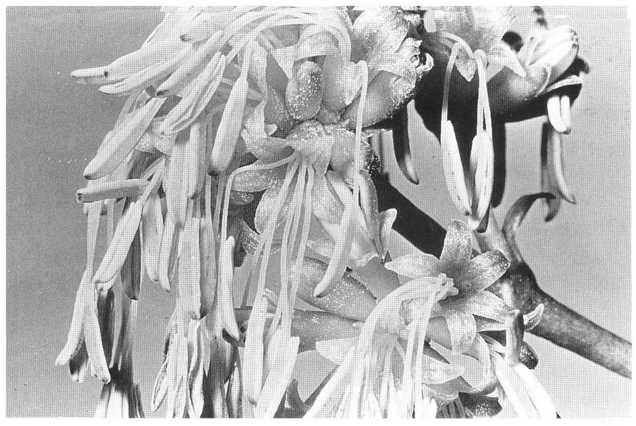
\includegraphics[width=0.66\textwidth]{graphics/figure5kanono.jpg}
	\centering
	\caption[Kanono: A New Zealand example of both wind pollination and dioecism]{\IDX{Kanono}[kanono] (\BotanicRef{Coprosma grandifolia}[Coprosma][grandifolia]): A New Zealand example of both wind pollination and dioecism.
	The flowers are male.
	As is generally the case with wind-pollinated flowers they are small and inconspicuous, but have disproportionately large dangling stamens with large anthers.
	The hanging stamens move readily with the wind, which shakes out the large quantities of pollen necessary for this rather wasteful method of pollination.
	The family to which \BotanicRef{Coprosma} belongs, the Rubiaceae, is mostly insect-pollinated with often showy flowers.
	The species of \BotanicRef{Coprosma} are unusual in the family in being both dioecious and wind-pollinated.
	Photo: M. D. King.}%
	\label{fig:5kanono}
\end{SCfigure}

Probably the isolated island characteristics in the New Zealand flora developed after isolation had been attained, and, more particularly, since high mountains and glacial/interglacial fluctuations have developed in recent geological times.
When mountains first became significant and temperatures cooled sufficiently the climate would have become too cold on the mountain tops for tree growth and alpine habitats would have come into existence like new islands, although in this case not surrounded by a sea of water, but by a sea of mostly unsuitable plants.
Because of New Zealand's isolation, plants suited to cold conditions elsewhere could arrive only slowly by long distance dispersal so there would have been plenty of opportunity for the establishment of hardy variants of forest genera in progressively colder habitats.
It was probably in these circumstances that genera such as \BotanicRef{Coprosma} attained their present, unusually wide, morphological and ecological ranges by radiating into non-forest habitats.

As each glacial phase progressed the area of alpine vegetation would extend, reaching sea level in many places.
The forests would become greatly restricted with some species becoming extinct and others barely surviving.
With the warmer conditions of the interglacials the situation would be reversed and the alpine flora would come under pressure.
Such climatic fluctuations, combined with an isolation that would prevent both the ready recruitment by long distance dispersal of species into new habitats, and the ready survival by migration of species already present, would put variable populations, including dioecious species and hybrid swarms, at a distinct advantage.
In times favourable to their vegetation type they would be best able to take advantage of new habitats and in unfavourable times they would be more likely to survive.

\section{Alternative Views}

The preceding analysis concludes that both long distance dispersal and former land connections have played a role in the ancestry of the New Zealand flora.
This would, I think, be the majority view at the present time, but there are alternatives: on the one hand Mildenhall\footnote{\cite{mildenhall1980new}} considers the possibility of long distance dispersal even for \BotanicRef{Nothofagus}, while on the other the `panbiogeographers' do not think speculation on dispersal has any value when trying to explain the presence of certain taxa on isolated islands.\footnote{\cite{craw1982phylogenetics}}

Alternatives to long distance dispersal as an explanation for the floras of isolated islands include the suggestion of Melville\footnote{\cite{melville1981vicarious}} and others that there was formerly a continent, Pacifica, which rifted into a number of fragments that drifted through the Pacific and eventually became incorporated into various continents on the Pacific rim.
If true, this would mean that the isolated central Pacific islands or their predecessors may have been close to continental fragments in the past and could have derived the nuclei of the present island floras from them.
It is further suggested that Pacifica was originally sited in the south-west Pacific and that it may have provided the sediments that now form the rocks of eastern New Zealand.

Carey\footnote{\cite{carey1983necessity}} has promoted a different idea for some time --- that the earth is expanding.
When it was much smaller all the present land areas were together without intervening oceans.
As the earth expanded the land areas moved apart and the new basins between them became filled with water derived from the earth's interior.
In this case too the islands of the young small Pacific Ocean could have derived their floras from the then nearby continents.

\section{Other Special Features of the Flora}

Other striking and puzzling features of the New Zealand flora will be considered in later chapters.
These include:

\begin{description}
	\item[{(a)}]the abundance of specialised growth forms in the conifer broad-leaf forests that are similar to growth forms of tropical forests;
	\item[{(b)}]the prevalence of distinct and varied juvenile forms in a number of the forest species;
	\item[{(c)}]the local abundance of very small-leaved, densely twiggy, springy, often cushion-like shrubs (divaricating shrubs) belonging to many species and ranging from forest and open lowland habitats to beyond tree line;
	\item[{(d)}]specialised alpine growth forms such as cushion plants and scree plants.
\end{description}
